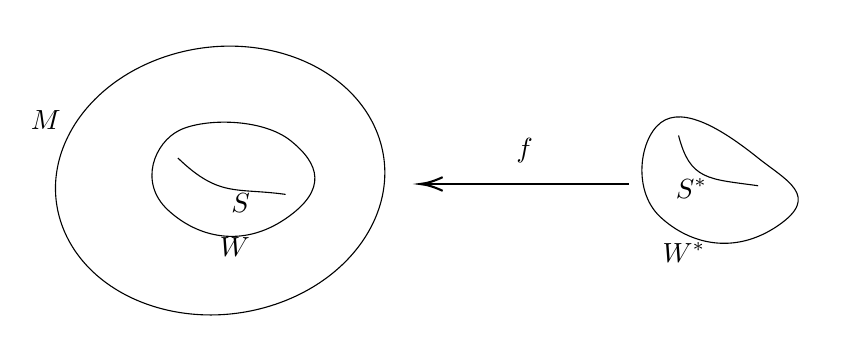
\begin{tikzpicture}[x=0.75pt,y=0.75pt,yscale=-1,xscale=1]
%uncomment if require: \path (0,223); %set diagram left start at 0, and has height of 223

%Shape: Ellipse [id:dp31205351375005885] 
\draw   (35.18,105.18) .. controls (21.37,71.95) and (43.89,34.3) .. (85.46,21.08) .. controls (127.04,7.86) and (171.93,24.08) .. (185.74,57.3) .. controls (199.54,90.53) and (177.03,128.18) .. (135.45,141.4) .. controls (93.87,154.62) and (48.98,138.4) .. (35.18,105.18) -- cycle ;
%Curve Lines [id:da6654336320515477] 
\draw    (90.09,70.38) .. controls (110.06,89.59) and (118.04,84.58) .. (142.01,87.92) ;
%Shape: Polygon Curved [id:ds6403319524310442] 
\draw   (90.89,57.01) .. controls (102.87,51.17) and (130.82,51.17) .. (144.4,62.03) .. controls (157.98,72.89) and (162.77,85.42) .. (142.01,99.62) .. controls (121.24,113.82) and (99.67,108.81) .. (85.3,95.44) .. controls (70.92,82.08) and (78.91,62.86) .. (90.89,57.01) -- cycle ;
%Shape: Polygon Curved [id:ds6985670513888118] 
\draw   (324.92,52) .. controls (336.9,46.15) and (356.07,59.52) .. (369.65,70.38) .. controls (383.23,81.24) and (400,88.76) .. (379.24,102.96) .. controls (358.47,117.16) and (336.9,112.15) .. (322.52,98.78) .. controls (308.15,85.42) and (312.94,57.85) .. (324.92,52) -- cycle ;
%Curve Lines [id:da37504253031609736] 
\draw    (331.31,59.52) .. controls (336.9,81.24) and (345.69,80.4) .. (369.65,83.75) ;
%Straight Lines [id:da1757973560387438] 
\draw    (307.35,82.91) -- (208.71,82.91) ;
\draw [shift={(206.71,82.91)}, rotate = 360] [color={rgb, 255:red, 0; green, 0; blue, 0 }  ][line width=0.75]    (10.93,-3.29) .. controls (6.95,-1.4) and (3.31,-0.3) .. (0,0) .. controls (3.31,0.3) and (6.95,1.4) .. (10.93,3.29)   ;

% Text Node
\draw (109.04,107.33) node [anchor=north west][inner sep=0.75pt]   [align=left] {$\displaystyle W$};
% Text Node
\draw (17.99,46.34) node [anchor=north west][inner sep=0.75pt]   [align=left] {$\displaystyle M$};
% Text Node
\draw (114.54,86.44) node [anchor=north west][inner sep=0.75pt]   [align=left] {$\displaystyle S$};
% Text Node
\draw (322.4,109.67) node [anchor=north west][inner sep=0.75pt]   [align=left] {$\displaystyle W^{*}$};
% Text Node
\draw (328.7,78.76) node [anchor=north west][inner sep=0.75pt]   [align=left] {$\displaystyle S^{*}$};
% Text Node
\draw (251.93,59.71) node [anchor=north west][inner sep=0.75pt]   [align=left] {$\displaystyle f$};


\end{tikzpicture}
